\chapter{Informationsbeschaffung}
\label{Informationsbeschaffung}
Im Rahmen der Projektplanung, welche in Anhang \todo{insert reference} ersichtlich ist, wurde in einer ersten Phase ein Zeitraum zur Informationsbeschaffung festgelegt. Dieser Abschnitt ist einerseits für die Themeneinarbeitung und anderseits für die Absteckung der Aufgabe und der Ziele erforderlich.

Nachfolgend werden die wichtigsten Erkenntnisse der Informationsbeschaffung erläutert, die maßgebend für die Konzeption in Kapitel \ref{chap:Konzeption} und die Realisierung in Kapitel \ref{chap:Realisierung} sind. Dabei werden zu einzelnen Komponenten und Verfahren Stellung genommen und eruiert, ob diese sich für das Projekt eignen. Des Weiteren werden relevante Software erläutert, welche für die Realisierung nötig sind. Das Projekt wurde dabei in verschiedene Funktionsblöcke unterteilt, die in den nachfolgenden Unterkapiteln beschrieben werden.


\section{Entfernungsmessung}
\label{sec:Entfernungsmessung}
In diesem Unterkapitel werden die bestehenden Entfernungsmesser Velodyne VLP-16 und der Hokuyo URG-LX01 detailliert betrachtet und die wichtigsten Spezifikation hervorgehoben. Es werden zusätzlich noch alternative Produkte gegenüber gestellt.

\subsection{Hokuyo URG-04LX}
\label{subsec:Hokuyo}
Der Hokuyo URG-04LX ist ein zweidimensionaler Entfernungsmesser, der mittels \ac{LIDAR} Verfahren misst. Bei diesem Verfahren werden mit reflektierten Laserimpulsen die Entfernung eruiert. Nachfolgende Angaben entstammen aus den Datenblättern. \todo{ref} 

Der Laserscanner bietet eine 

\begin{figure}[H]
	\centering
	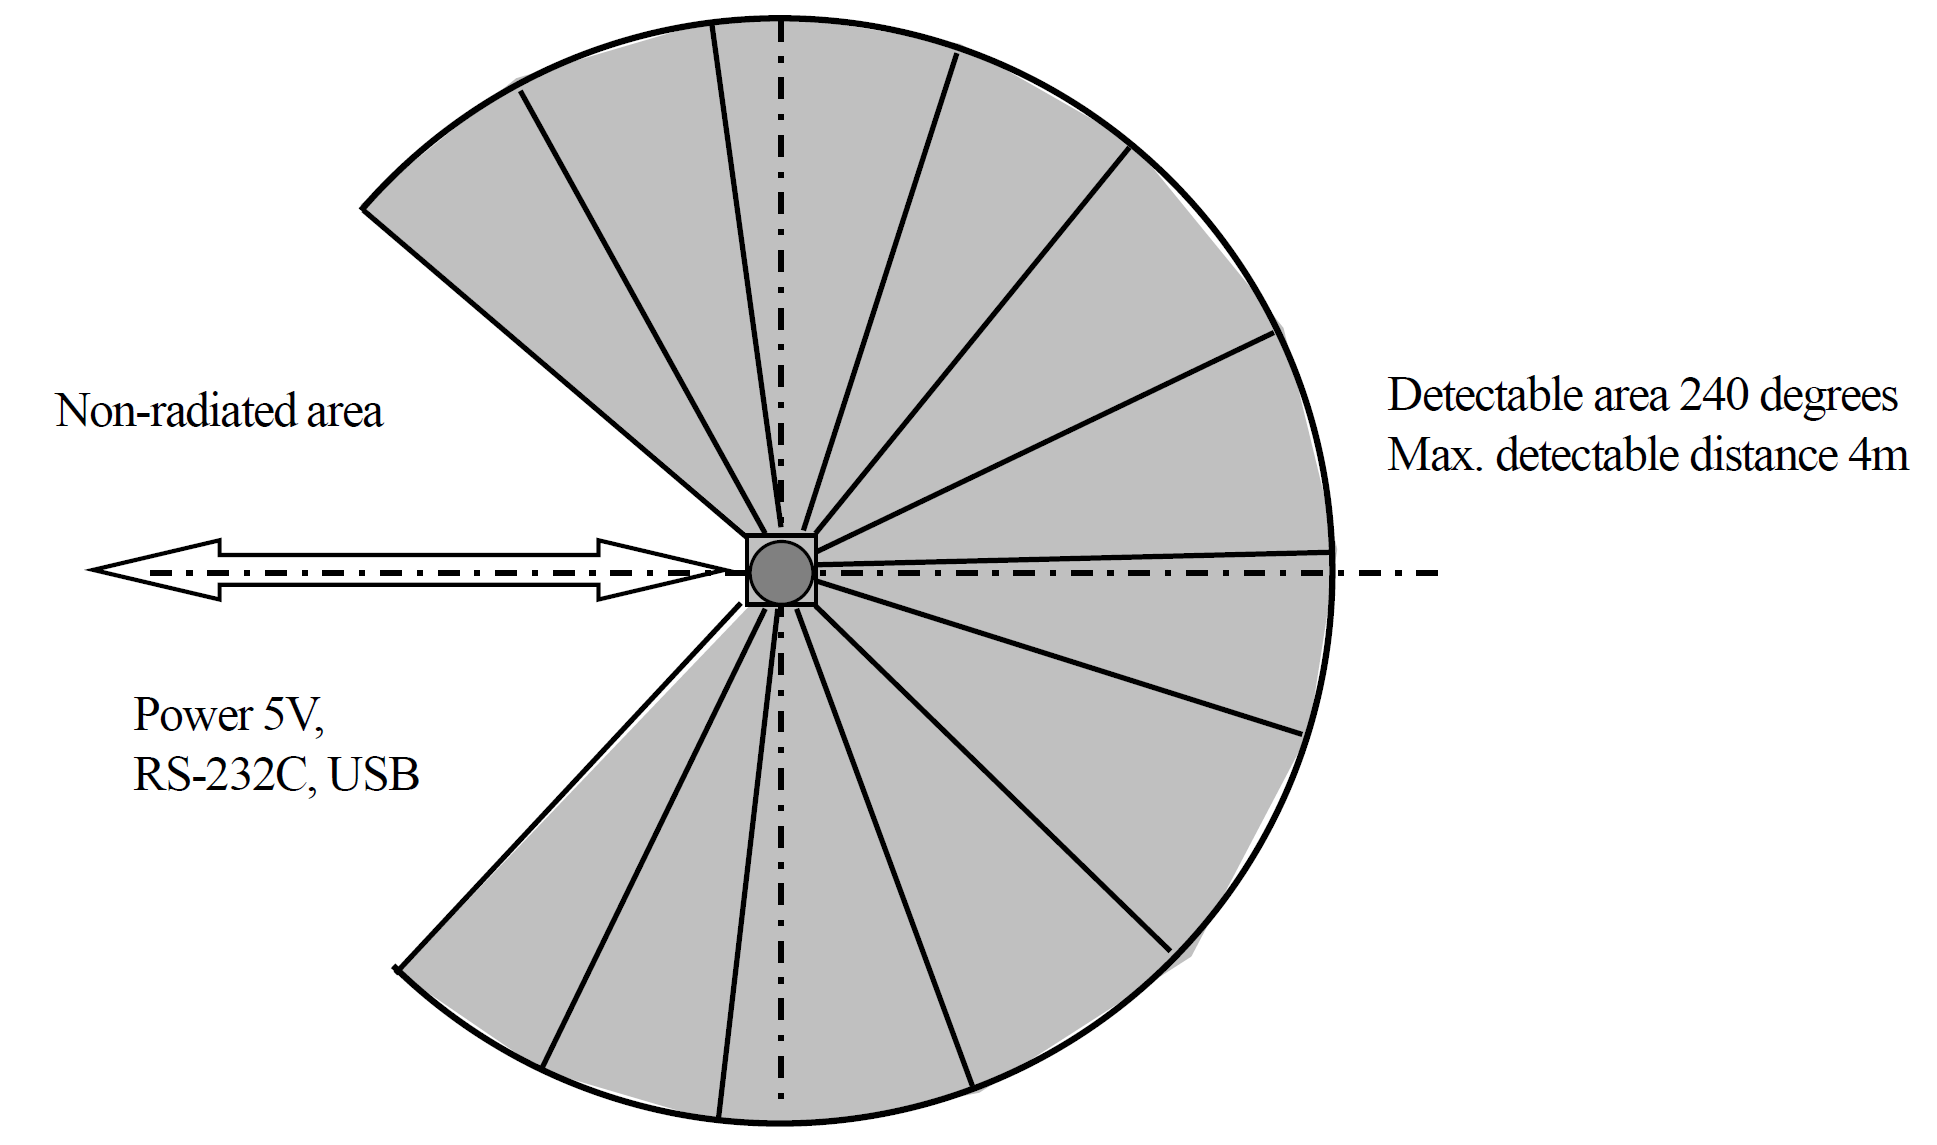
\includegraphics[width=0.5\textwidth]
	{resources/detectableAngle.PNG}
	\caption[detektierbarer Winkel]{detektierbarer Winkel} \protect\cite{Hokuyo}
	\label{fig:URG-04LX}
\end{figure}

\todo{ref}
Ein bedeutendste Nachteil des URG-04LX für die Aufgabenstellung ist das messbare Distanzspektrum. Die maximale Messdistanz von 4 Meter genügt nur für sehr nahe räumliche Messungen. Der Einsatzbereich beschränkt sich hier lediglich für Gebäude interne Messungen.

\subsection{Velodyne VLP-16 Puck}
\label{subsec:Velodyne}
Beim Velodyne VLP-16 Puck handelt es sich um einen Echtzeit 3D-Laser-Scanner, der auf dem \ac{LIDAR}-Verfahren basiert. Nachfolgende Angaben entstammen den Datenblattangaben, wenn nicht anders referenziert.

Der VL

\begin{figure}[H]
	\centering
	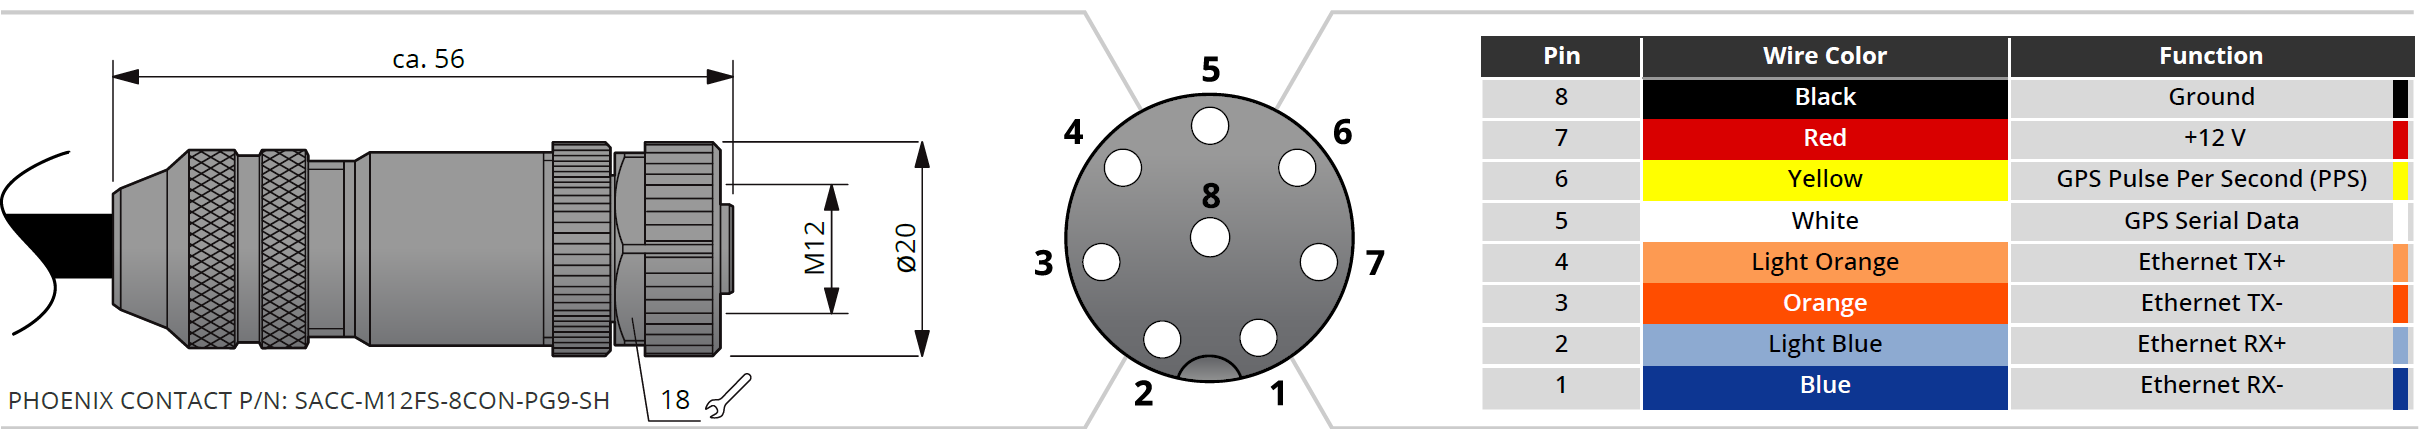
\includegraphics[width=1\textwidth]{resources/Cablepins.PNG}
	\caption[Anschluss und Kabelbelegung]{Anschluss und Kabelbelegung}
	\label{fig:CablePin}
\end{figure} 

Der Velodyne benötigt eine seperate Interface Box, da die Speisung und Datenübertragung des 8-adriges Anschlusskabel getrennt werden muss. In \ref{fig:Cablepin} ist dieses Kabel mit Pinbelegung dargestellt. Die Interface Box ist in \ref{fig:InterfaceBox}  Diese besitzt die 12 Volt Speisung, sowie ein Ethernet RJ45 Anschluss und eine \ac{GPS} Schnittstelle, damit . Die typische Leistungsaufnahme des Sensors ist hierbei 8 Watt.

\begin{figure}[H]
	\centering
	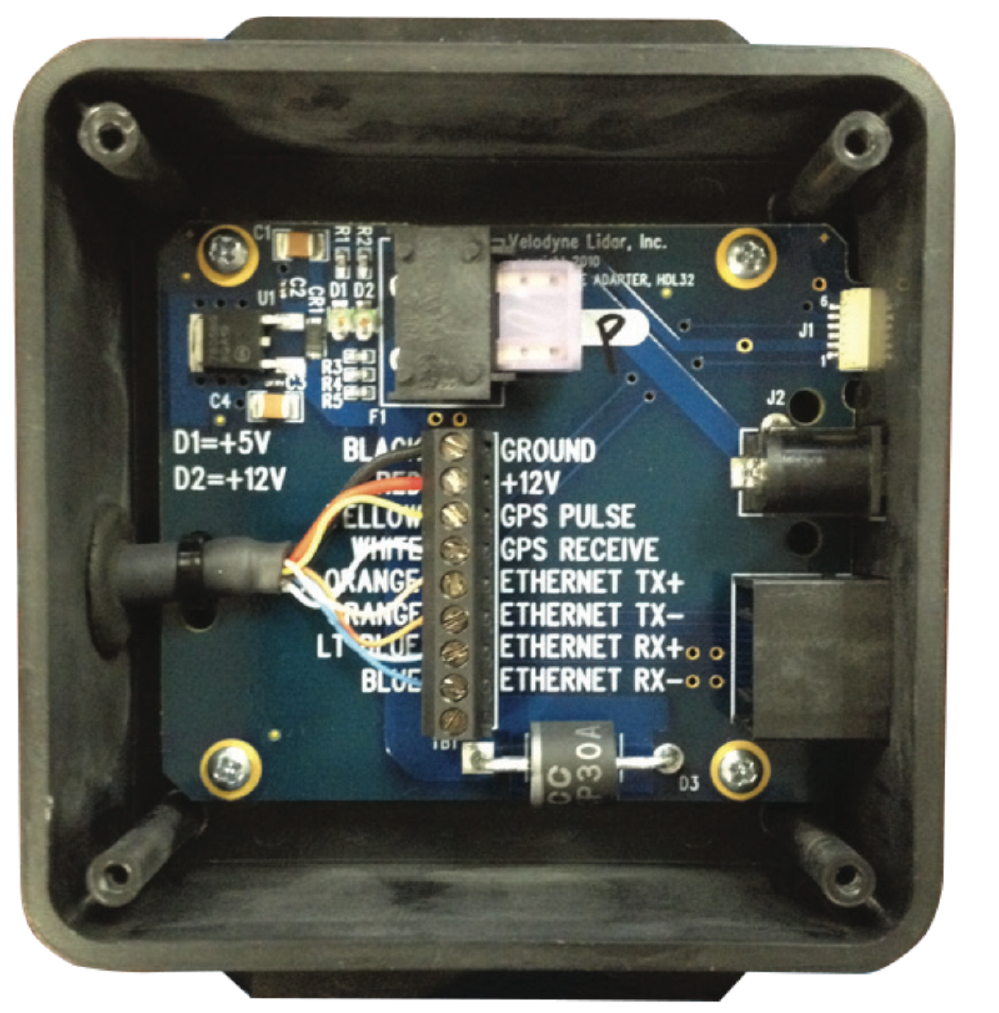
\includegraphics[width=0.4\textwidth]
	{resources/InterfaceBox.PNG}
	\caption[Ansichct auf die Interfacebox]{Ansicht auf die Interface Box} \protect\cite{Velodyne}
	\label{fig:InterfaceBox}
\end{figure}



\subsection{Alternativen zu LIDAR}
 \label{subsec:Alternative}
 
 \todo{evlt erweitern}
 

\section{Software}
\label{sec:Software}
In diesem Kapitel wird die notwendige Software beschrieben. Es erläutert einerseits das ROS und dessen Funktion im Projekt. Daneben werden kurz weitere Sofwareapplikationen und -packages erwähnt, welche während der Erarbietung hilfreich sind.

\subsection{ROS Robot Operating System}
\label{subsec:ROS}
Die gesamte Kommunikation mit Sensoren und Aktoren findet auf dem Packbot mit einem spezifisch implementierten \ac{ROS} statt. Daher ist es naheliegend, um die Integrität des zu erarbeitenden 3D-Laser-Moduls zu gewährleisten, dieses Software-Framework zu nutzen.  

\subsection{ROS Kinetic Kame vs. Indigo}
\label{subsec:OS_versus} 
Grundsätzlich wird ROS, wegen seiner Nähe zu Linux Distributionen, auf einem Ubuntu Betriebssystem aufgesetzt und ist ein grösstenteils Kommando-basiertes Software-Framework. Diese in 2007 entwickelte Open Source Software erhielt in den letzten Jahren ständig neue und überarbeitete Versionen. In der nachfolgenden Abbildung sind die aktuellen Distributionen ersichtlich.

\begin{figure}[H]
	\centering
	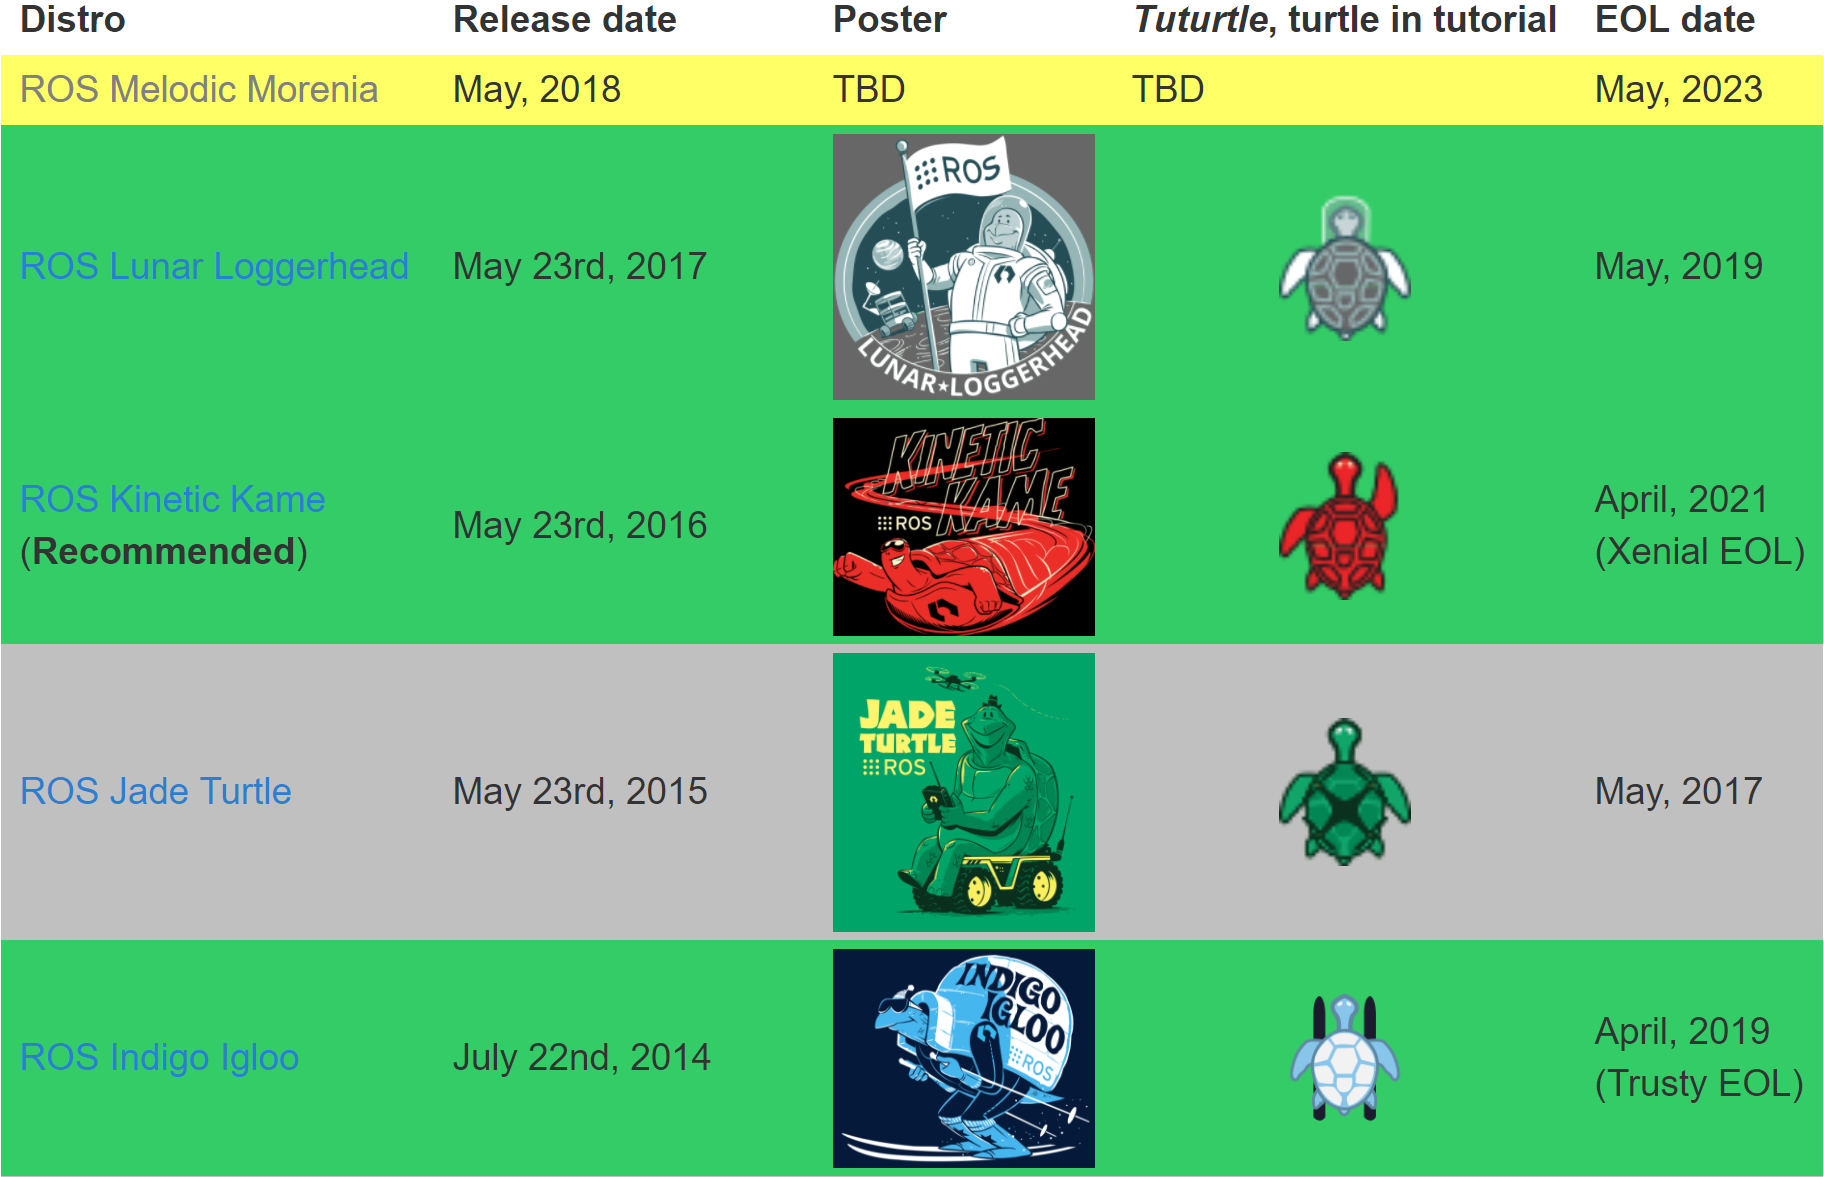
\includegraphics[width=0.6\textwidth]{resources/rosdistos.PNG}
	\caption[aktuelle Disttributionen von ROS]{aktuelle Disttributionen von ROS {\cite{ROSprojects}}}
	\label{fig:rosdistros}
\end{figure} 

Die Empfehlung von ROS und diversen Literaturen liegt hierbei bei der neusten Distribution ROS "Kinetic Kame". Es handelt sich hierbei um eine Langzeitversion von ROS, welche bis 2021 unterstütung bietet. Im Zug der ersten Versuchen mit ROS wurde auf einem Laptop mit AMD64-Architektur gearbeitet. Auf diesem wurde ROS Kinetic Kame vollumfänglich ermöglicht. Für das 3D-Lasermodul wird jedoch ein einbaubaren Einplatinencomputer benötigt, welche im \ref{sec:Datenverarbeitung} genauer betrachtet werden. 

Während der Einarbeitung mit Kinetik Kame konnten einige Nachteile der Distirbution festgestellt werden. Kinetik Kame unterstützt offiziell die erforderliche Velodyne Packages für den VLP-16 noch nicht. Diese können jedoch über einen unoffiziellen Github Account von DataSpeed Inc. bezogen werden. Dabei wurde jedoch festgestellt, dass diese unoffiziellen Packages nur für amd64-Architekturen zur Verfügung stehen. Dies ist ein wesentlicher Nachteil, da die meisten Einplatinencomputer mit ARM-Architekturen arbeiten.
\todo{Erkentnisse 01.11.2017}

Der Vorgänger ROS Indigo unterstützt offiziell die Velodyne Packages. Dabei muss jeodch berücksichtigt werden, dass Indigo nur auf Ubuntu 14.04 Trusty Truh. ROS Indigo wird nur noch bis April 2019 unterstützt, bietet jedoch im Vergleich zu allen Distributionnen die meisten offiziellen Packages, da es bereits 2014 veröffentlicht wurde.

\subsection{Point Cloud Library}
\label{subse:PointCloudLibrary}
Die Point Cloud Library (PCL) ist eine freie Programmbibliothek mit zahlreichen Algorithmen zur Verarbeitung n-dimensionaler Punktwolken und dreidimensionaler Geometrien.

Ein wesentlicher Vorteil dieser Programmbibliothek ist die Integration in ROS.
\subsection{Wireshark}
\label{subcec_Wirehark}
\todo{evlt}
\subsection{Onshape}
\label{subsec:OnShape}
\todo{evlt}

\section{Datenverarbeitung}
\label{sec:Datenverarbeitung}
Um die enorme Datenmenge zu verarbeiten muss eine entsprechende leistungsstarker Prozessor zur Verfügung stehen. Es wurden diverse Einplatinencomputer betrachtet und folgende Erkenntnisse daraus gezogen.

\subsection{Raspberry Pi 2 \& 3}
\label{subsec:Raspberry}
Das Raspberry Pi ist eines der bekanntesten Einplatinencomputer und bietet daher eine grosse Community. Da bereits ein Raspberry Pi 2 zur Verfügung gestanden ist, konnten die ersten Erfahrungen mit einem Raspberry Pi gemacht werden. Das Raspberry bietet zusammen mit ROS Kinetic Kame und Ubuntu Mate LTS 16.04 eine mögliche Lösung für die Datenverarbeitung. Das Raspberry Pi 2 bzw. 3 basiert auf einem Broadcom \ac{SOC}, ist mit einem ARM Cortex A7 bzw. A53 Prozessor ausgestattet. Dabei wird der Speicher auf einer \ac{SD}-Card  gebootet. 

\subsection{Banana Pi M3}
\label{sec:BananaPi}
Der Banana Pi M3 bietet zur Zeit (Stand Oktober 2017) die höchste Performance bei Einplatinencomputern mit ARM-Architekture, durch den Allwinner A83T Achtkern-Prozessor. Neben USB-Anschlüssen bietet er eine SATA-USB-Schnittstelle, die den internen 8 GB Speicher um bis zu 2 TB erweitern lässt, direkt integrierte Schnittstellen wie Bluetooth und WLAN, sowie eine RJ45 Gigabit Netzwerkschnittstelle. Zum Betreiben des Banana PI-M3 benötigen man ein 5V DC-Netzteil. Der Preis eines BananaPi M3 liegt momentan bei ca 90. Franken.

 
\subsection{Odroid C2 \& XU4} 
\label{Odroid}
In diversen Literaturen (siehe \cite{ROSprojects} Kapitel 4) werden neben dem Raspberry Pi, das Odroid Board als empfohlene Einplatinencomputer aufgelistet. Dabei stehen die aktuelle Modelle Odroid-C2 oder Odroid-XU4 zur Verfügung. Sie bieten eine höhere Prozessorleistung, 1.5GHz bzw. 2GHz mit je 2 Gigabyte \ac{RAM}. Beide Boards sind jedoch noch nicht lange auf dem Markt und bieten in vielen Anwendungen nur Beta-Versionen. Vor allem die Unterstützung von Ubuntu LTS 16.04 ist nicht restlos gekärt. Der Preis dieser Boards ist um die 80 - 90 Franken.

\subsection{Lattepanda} 
\label{Lattepanda}
Der Lattepanda Einplatinencomputer unterscheidet sich wesentlich von den bisherig betrachteten Baords. Der Prozessor arbeitet nicht mit ARM-Architekture, sondern mit AMD64-Architekture und 


\section{Antriebsmöglichkeiten}
Um das Produkt um eine Achse drehen zu lassen, müssen Motoren eingesetzt werden. Nachfolgend sind zwei verschiedene Motorenarten geschildert, um die Einsatzmöglichkeit zu klären. Wichtige Kriterien für die Aufgabenstellung sind einerseits die Ansteuerung und die Dimension. Anderseits muss die Möglichkeit bestehen die Winkeländerung zu eruieren. 

\subsection{Schrittmotor}
Der Schrittmotor ist eine Antriebsmöglichkeit, welche für das Projekt in Frage kommt. Es gibt sehr kostengünstige und kompakt dimensionierte Motoren dieser Art. Ein interessanter Aspekt ist das  gezielt steuern des Motors. Durch einen Stromimpuls bewegt sich ein Schrittmotor nur einen festgelegten Winkelschritt weiter. Er kann bereits ohne zusätzliche Sensorik definierte Schritte anfahren, aus denen die Winkeländerung eruiert werden kann. Schrittmotoren besitzen die Eigenschaft, dass in der Ruhelage ein Haltemoment entsteht. Diese Eigenschaft wird jedoch für die Aufgabenstellung nicht zwingend benötigt.

Nachteilig für die Aufgabenstellung am Schrittmotor ist der höhere Stromverbrauch, vor allem während dem Haltemoment. Da nur ein Schritt vollführt werden kann, wenn das entsprechende Drehmoment nicht überschritten wird, müsste dieses sorgfältig berechnet werden. Ein bedeutender Nachteil im Zusammenhang mit der Aufgabenstellung ist, dass durch Schrittverluste die Winkeländerung nicht mehr quantitativ ermittelt werden kann.
Ein weiterer Nachteil ist das verhältnismäßig hohe Gewicht. Dies ist kein Kriterium für die Aufgabenstellung, sollte jedoch bei der Realisierung beachtet werden.

Um mit einem Mikrocontroller einen Schrittmotor anzusteuern, empfiehlt sich ein Motorentreiber benötigt. Mit solchen Treibern lässt sich der Motor mittels 2 Steuerpins rotieren. Um die Drehgeschwindigkeit zu senken, bieten diese Treiber die Möglichkeit, die Schritte in 2, 4, 8 und 16 Teilschritte zu senken,um dadurch eine feinere Bewegung zu ermöglichen. 

\subsection{Gleichstrommotor}
Als Alternative zum Schrittmotor bietet sich ein üblicher Gleichstrommotor. Diese Motoren sind für viele Einsatzbereiche geeignet und es gibt sie in verschiedenen Grössen und Umdrehungszahlen. Im Gegensatz zu Schrittmotoren laufen DC-Motoren kontinuierlich, aufgrund eines Stroms, der durch die Wicklungen fliesst. Nachteilig ist somit, dass weder die genaue Anzahl Umdrehungen noch die momentane Phasenlage bekannt ist. Es gibt jedoch eine Vielzahl an Möglichkeiten diese zu eruieren. Einerseits gibt es die Möglichkeit mittels Hall-Sensoren oder mittels Quadraturencodern den  Um dies zu ermöglichen, braucht es zusätzlich einen Vierquadrantensteller (H-Brücke), sowie eine Sensorlogik, welche die Umdrehung misst. Im Preissegment bis 40 Fr. gibt es leistungsfähige Gleichstrommotoren

\subsection{Abwärtswandler}
Der Abwärtswandler D24V50F5 von Pololu eignet sich sehr gut für die Stromversorgung von Einplatinencomputer. Er bietet eine stabil 5V-Ausgangsspannung bis zu einer ausgangsseitigen Belastung von 8 Ampere. Der Wirkungsgrad beläuft dabei auf knapp über 90 Prozent bei einer eingesetzten Betriebsspannung von 12 Volt. Diese Angaben gehen aus Abbildung \ref{fig:D24V50F5} hervor, die aus dem Datenblatt des  

\begin{figure}[H]
	\centering
	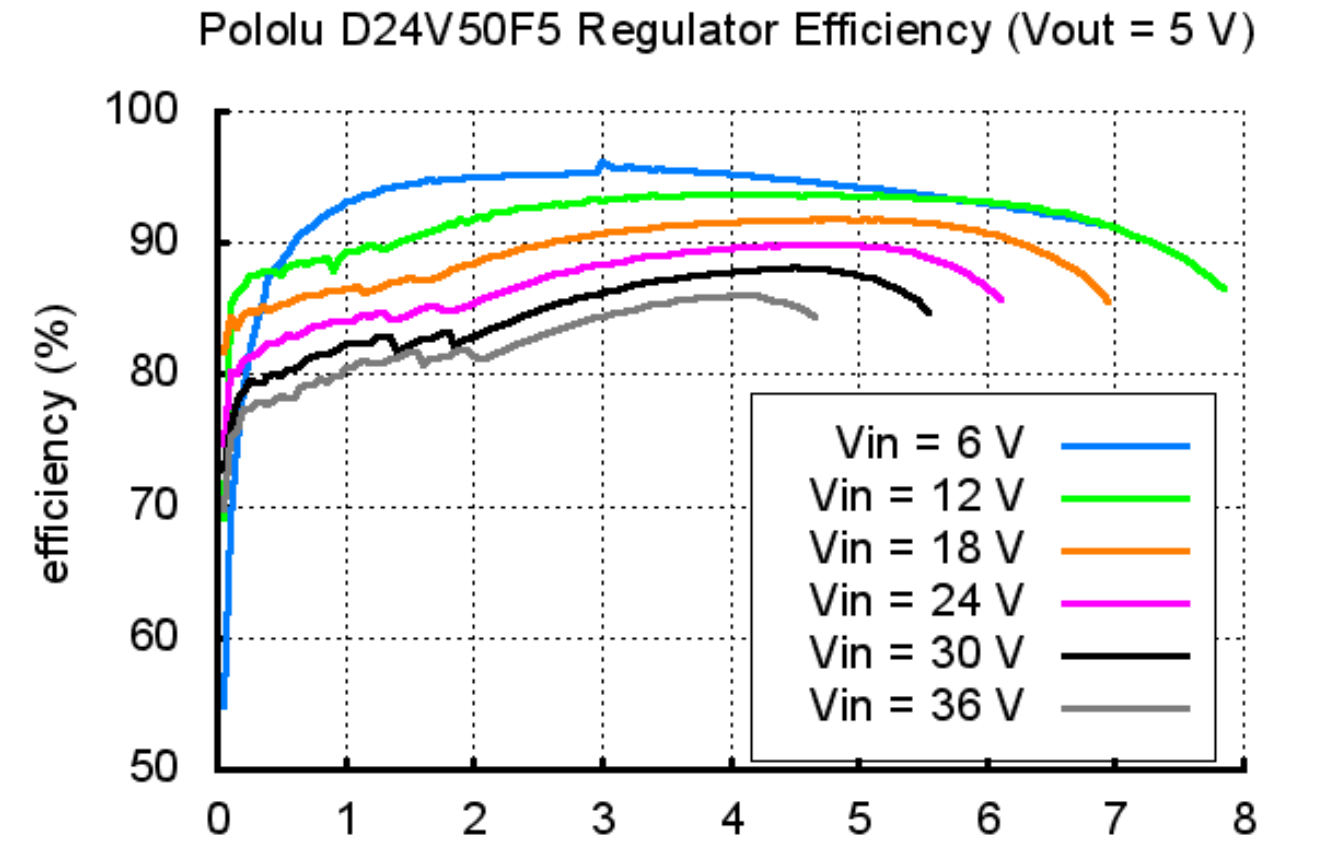
\includegraphics[width=0.5\textwidth]
	{resources/D24V50F5.PNG}
	\caption[Wirkungsgrad D24V50F5]{Wirkungsgrad D24V50F5 \protect\cite{D24V50F5}}
	\label{fig:D24V50F5}
\end{figure}



\section{Zwischenfazit}
\label{ZwischenfazitInfo}
Für die Einarbeitung in das Projekt ist die Informationsbeschaffung bzw. Recherche ein wesentlicher Bestandteil. Dabei werden wichtige Grundlagen für die Konzeption erstellt. Mittels Schrittmotoren oder Gleichstrommotoren kann der Velodyne gedreht werden. Für die Datenverarbeitung stehen mehrere Einplatinencomputer zur Verfügung, dabei muss jedoch die Integration in das System gewährleistet sein. Für 3D Mapping gibt es  